\documentclass[sigconf]{webmedia}

\AtBeginDocument{%
  \providecommand\BibTeX{{%
    \normalfont B\kern-0.5em{\scshape i\kern-0.25em b}\kern-0.8em\TeX}}}

\settopmatter{printacmref=false, printfolios=false}

%% Evento
\setevent{webmedia}
\proceedingsDetails[WebMedia’2026]{Proceedings of the Brazilian Symposium on Multimedia and the Web}{2026}{Lavras/MG, Brazil}
\ISSN{2966-2753}

%% Marcador de pendências
\newcommand{\TODO}[1]{\textbf{[PREENCHER: #1]}}
%% Inclui a tabela gerada pelos scripts; se ainda não existir, mostra um aviso
\newsavebox{\tabbox}
\newcommand{\tabela}[2]{%
  \sbox{\tabbox}{\InputIfFileExists{#1}{}{\TODO{rodar #2}}}%
  \ifdim\wd\tabbox>\linewidth
    \resizebox{\linewidth}{!}{\usebox{\tabbox}}%
  \else
    \hbox to \linewidth{\hfil\usebox{\tabbox}\hfil}%
  \fi}

\begin{document}

\title[Análise Estrutural do Grafo com-Youtube]{Análise Estrutural e Algorítmica da Rede Social do YouTube}

\author{Lucas Costa Soares}
\email{lucas.srs@ufba.br}
\affiliation{
  \institution{Universidade Federal da Bahia - UFBA}
  \city{Salvador}
  \country{Brasil}}

\renewcommand{\shortauthors}{Soares}

\begin{abstract}
Este trabalho analisa a rede social \texttt{com-Youtube}, disponibilizada pelo projeto SNAP, por meio de (i) medidas estruturais clássicas, (ii) algoritmos de grafos da disciplina, comparando complexidade teórica e tempo observado com intervalos de confiança, e (iii) propriedades de redes complexas: efeito \emph{small-world}, lei de potência na distribuição de graus e robustez a falhas aleatórias e ataques direcionados. A rede tem 1\,134\,890 vértices, grau médio $\approx 5{,}3$, caminho médio $\approx 5{,}4$ e diâmetro 24, com clusterização média 0,081 muito acima da de um grafo aleatório equivalente, o que caracteriza o efeito \emph{small-world}. A distribuição de graus tem cauda pesada ($\gamma\approx 2{,}1$ por máxima verossimilhança). A rede resiste bem à remoção aleatória de 5\% dos vértices (maior componente com 91\% dos vértices), mas é muito vulnerável a ataques direcionados (29\% e 25\% para grau e PageRank).
\end{abstract}

\keywords{análise de redes, grafos, small-world, lei de potência, robustez, algoritmos de grafos}

\maketitle

%% =====================================================================
\section{Introdução}
Redes sociais \emph{online} apresentam estrutura não trivial, com poucos vértices muito conectados e agrupamento local elevado. Neste trabalho, é estudada a rede de amizades do YouTube (\texttt{com-Youtube}) \cite{yang2015defining,snapnets}. Entender essa estrutura ajuda a explicar como informação e influência se propagam e quão frágil a rede é diante da perda de usuários centrais.

A contribuição deste trabalho é um estudo reprodutível em três partes: (I) medidas estruturais exatas ou estimadas, com indicação explícita do que foi aproximado; (II) implementações próprias de algoritmos clássicos de grafos, com comparação entre complexidade teórica e tempo observado; e (III) testes de \emph{small-world}, de lei de potência e de robustez.

O texto segue esta ordem: a Seção~\ref{sec:grafo} descreve o grafo original, incluindo a sua determinação, a descrição do conjunto de dados e o tratamento dos dados; a Seção~\ref{sec:metodologia} apresenta a metodologia de todas as partes; as Seções~\ref{sec:parte1} a~\ref{sec:parte3} trazem os resultados das Partes~I a~III; a Seção~\ref{sec:discussao} faz a discussão crítica; e a Seção~\ref{sec:conclusao} conclui.

%% =====================================================================
\section{Descrição do Grafo Original}
\label{sec:grafo}

\subsection{Determinação do Grafo}
\label{sec:determinacao}
O grafo a ser analisado por cada aluno é determinado a partir do número de matrícula $M$, pela fórmula
\begin{equation}
  g = \bigl(S(M)\cdot(U(M)+1)\bigr) \bmod 129,
\end{equation}
em que $S(M)$ é a soma dos dígitos de $M$ e $U(M)$ é o número formado pelos dois últimos dígitos de $M$. Para a matrícula $224215940$ tem-se $S=2+2+4+2+1+5+9+4+0=29$ e $U=40$, logo $g=(29\cdot 41)\bmod 129=1189\bmod 129=28$. O índice 28 corresponde ao grafo \href{https://snap.stanford.edu/data/com-Youtube.html}{\texttt{com-Youtube}}, analisado neste trabalho.

\subsection{O Conjunto de Dados \texttt{com-Youtube}}
\label{sec:conjunto}
O \texttt{com-Youtube} é a rede social do YouTube, um serviço de compartilhamento de vídeos que inclui uma rede social: cada vértice é um usuário e cada aresta é uma relação de amizade, de modo que o grafo é não direcionado e não ponderado. Os dados foram fornecidos por Mislove et al.\ \cite{mislove2007} e são distribuídos pelo SNAP \cite{snapnets,yang2015defining}. Além do grafo, o SNAP disponibiliza 8\,385 comunidades de \emph{ground-truth}, definidas a partir dos grupos criados pelos usuários (cada componente conexa de um grupo é uma comunidade e as com menos de 3 vértices são removidas); elas não foram usadas, pois este trabalho analisa apenas a estrutura do grafo.

Quanto ao recorte, o SNAP distribui \textbf{apenas a maior componente conexa}. Por isso o grafo tem uma única componente, com 100\% dos vértices e das arestas, e propriedades como número de componentes ou de vértices isolados não descrevem a rede completa do YouTube. A Tabela~\ref{tab:snap} compara as estatísticas publicadas pelo SNAP com as obtidas neste trabalho.

\begin{table}
  \caption{Estatísticas publicadas pelo SNAP e valores obtidos neste trabalho.}
  \label{tab:snap}
  \small
  \begin{tabular}{lrr}
    \toprule
    Medida & SNAP & Obtido \\
    \midrule
    Vértices & 1\,134\,890 & 1\,134\,890 \\
    Arestas & 2\,987\,624 & 2\,987\,624 \\
    Clusterização média & 0,0808 & 0,0808 \\
    Triângulos & 3\,056\,386 & 3\,056\,386 \\
    Diâmetro & 20 & 24 \\
    Diâmetro efetivo (90\%) & 6,5 & não calculado \\
    \bottomrule
  \end{tabular}
\end{table}

Vértices, arestas, clusterização e triângulos coincidem, o que valida a leitura e a limpeza dos dados e o cálculo de triângulos. O diâmetro difere: o SNAP informa 20 (a página não detalha o método), enquanto encontramos 24 por BFS. Como o valor 24 foi observado entre um par real de vértices, o diâmetro do grafo é pelo menos 24, e o valor de 20 do SNAP subestima o diâmetro, o que é compatível com uma estimativa por amostragem. O diâmetro efetivo (90-percentil das distâncias) não foi calculado; o caminho médio estimado (5,36) é coerente com o valor 6,5 do SNAP, já que o percentil 90 das distâncias é maior que a média.

\subsection{Responsabilidade pelo Tratamento dos Dados}
\label{sec:dados}
\paragraph{Origem e licença.} Os dados são públicos e foram obtidos diretamente do SNAP (arquivo \texttt{com-youtube.ungraph.txt.gz}). Os identificadores dos usuários já são anonimizados na origem e nenhuma tentativa de reidentificação foi feita.

\paragraph{Limpeza.} O tratamento foi feito de forma automática e reprodutível: (1) comentários do cabeçalho ignorados; (2) laços (arestas $u=u$) removidos; (3) arestas duplicadas e em sentidos opostos unificadas, tratando o grafo como simples e não direcionado; (4) identificadores originais, não contíguos, mapeados para $0,\dots,n-1$ (o mapeamento é preservado); (5) armazenamento em lista de adjacência compacta (CSR). O arquivo tinha 2\,987\,624 linhas; nenhum laço e nenhuma aresta duplicada foi encontrado, resultando em 1\,134\,890 vértices e 2\,987\,624 arestas. Nenhuma aresta ou vértice válido foi descartado ou alterado.

\paragraph{Reprodutibilidade e ferramentas.} Sementes aleatórias fixas (\texttt{GRAPH\_SEED}=42) garantem reprodutibilidade. Python com NumPy, NetworkX \cite{hagberg2008} (visualização e validação cruzada) e, opcionalmente, igraph \cite{igraph} (contagem exata de triângulos). Os algoritmos da Parte~II e as medidas de \emph{small-world} foram implementados do zero e validados contra o NetworkX em subgrafos (todas as comparações concordaram). Os scripts e resultados obtidos estão disponíveis no repositório do GitHub: \url{https://github.com/LucasC-Soares/YoutubeGraph}.

%% =====================================================================
\section{Metodologia}
\label{sec:metodologia}

\subsection{Parte I - Análise Estrutural}
O grafo foi tratado como simples e não direcionado e armazenado em lista de adjacência compacta (CSR). Grau (mínimo, máximo, médio e mediana), densidade, distribuição de graus e número e tamanho das componentes conexas são calculados de forma \emph{exata}. As medidas dependentes de caminhos (diâmetro, raio e caminho médio) são calculadas na maior componente conexa e, por terem custo proibitivo para todos os pares de vértices, são estimadas por BFS a partir de fontes amostradas: o diâmetro é um \emph{limite inferior} (maior excentricidade observada em 300 BFS), o raio é um \emph{limite superior} (menor excentricidade observada em 250 BFS) e o caminho médio é a média das distâncias a partir de 200 fontes, com IC95\%. A clusterização média e o número de triângulos foram calculados de forma exata com o igraph. A Tabela~\ref{tab:computado} indica, para cada medida, se ela foi calculada de forma exata, estimada ou não calculada, com justificativa.

\subsection{Parte II - Algoritmos da Disciplina}
Foram implementados BFS, DFS, verificação de eulerianidade, Dijkstra, Bellman-Ford, Floyd-Warshall, Tarjan (pontes e pontos de articulação) e árvore geradora mínima (Kruskal com união-busca e Prim) \cite{cormen2009,tarjan1972}. Em grafo não direcionado, as componentes fortemente conexas coincidem com as conexas, por isso Tarjan é aplicado a pontes e articulações.
Todas as implementações são próprias (iterativas, sem bibliotecas de grafos) e foram validadas contra o NetworkX em subgrafos.

\paragraph{Aplicabilidade.} O grafo é não ponderado e sem arestas de peso negativo: Dijkstra e Bellman-Ford equivalem à BFS e Floyd-Warshall é inviável no grafo inteiro ($O(V^3)$). Mesmo assim, para a comparação teórica$\times$observada, foram executados sobre subgrafos com pesos inteiros aleatórios em $[1,10]$ (semente fixa).

\paragraph{Medição de tempo.} Cada algoritmo foi executado $R$ vezes sobre subgrafos induzidos diferentes (bolas BFS de $V$ vértices em torno de fontes aleatórias) e, quando necessário, com fonte aleatória. Reportam-se média $\bar{x}$, desvio padrão $s$ e IC95\%:
\begin{equation}
  \bar{x}\pm z_{\alpha/2}\frac{s}{\sqrt{R}}\ (R\ge 30),\qquad
  \bar{x}\pm t_{\alpha/2,R-1}\frac{s}{\sqrt{R}}\ (R<30),
\end{equation}
com $z_{0{,}025}=1{,}96$. Foram usadas $R=30$ repetições por tamanho, logo a distribuição normal (Z) em todas as linhas da Tabela~\ref{tab:tempos}. Já as execuções no grafo completo usam $R=5$, e portanto a $t$ de Student com 4 graus de liberdade ($t_{0{,}025,4}=2{,}776$).

\paragraph{Complexidade observada.} Para comparar com a teoria, ajusta-se por regressão log-log $t\approx c\,f(V,E)^b$, em que $f$ é o custo teórico do algoritmo (Tabela~\ref{tab:complexidade}); $b\approx1$ indica que o tempo cresce como previsto.

\subsection{Parte III - Análise Estrutural Avançada}
\paragraph{Small-world.}
Um grafo é \emph{small-world} se $L(G)\approx L_{rand}$ e $C(G)\gg C_{rand}$, onde o grafo aleatório de referência tem o mesmo número de vértices e o mesmo grau médio. Utiliza-se um $G(n,m)$ de Erdős--Rényi \cite{erdos1959} gerado e medido pelo mesmo código, além dos valores teóricos $L_{rand}\approx\ln n/\ln\langle k\rangle$ e $C_{rand}\approx\langle k\rangle/n$, e o índice $\sigma=(C/C_{rand})/(L/L_{rand})$ \cite{watts1998}. A implementação é própria (sem bibliotecas de cálculo de \emph{small-world}).
Como a implementação é própria, a clusterização foi estimada em uma amostra de 20\,000 vértices e o caminho médio por BFS amostradas, ambos com IC95\%; o grafo de referência é gerado com o mesmo número de vértices e arestas, e as medidas são feitas na sua maior componente.

\paragraph{Lei de potência.}
Verifica-se se $P(k)\sim k^{-\gamma}$ com $\gamma>1$ por (i) gráficos log-log de $P(k)$ e da CCDF, (ii) regressão linear de $\log P(K\ge k)\times\log k$ e (iii) estimador de máxima verossimilhança de $\gamma$ com $k_{min}$ escolhido por mínima distância de Kolmogorov--Smirnov \cite{clauset2009}. Utiliza-se a aproximação contínua com correção de $1/2$ para dados discretos; \textbf{não} foi realizado o teste de bondade de ajuste por \emph{bootstrap} nem a comparação com outras distribuições de cauda pesada, o que limita a conclusão a \emph{indícios}.

\paragraph{Robustez.}
Seguindo o apêndice do enunciado, trabalha-se na maior componente conexa, com $r=\lceil 0{,}05\,n\rceil$ vértices removidos. As métricas são: (A) fração $S$ do grafo original na maior componente; (B) número de componentes; (C) caminho médio e limite inferior do diâmetro (BFS amostradas); (D) fração de nós isolados. Na remoção aleatória foram feitas $T=30$ repetições (média $\pm$ desvio, boxplots). No ataque direcionado, são removidos os $r$ vértices de maior centralidade de grau e de PageRank (ranking fixo, calculado uma vez). A betweenness exata é inviável neste porte, e o enunciado admite grau como alternativa.

%% =====================================================================
\section{Parte I - Análise Estrutural}
\label{sec:parte1}
A Tabela~\ref{tab:estrutural} reúne todas as medidas exigidas e a Tabela~\ref{tab:componentes} o tamanho das maiores componentes; a Tabela~\ref{tab:computado} indica quais foram calculadas de forma exata, estimada ou não calculadas. A Figura~\ref{fig:graus} mostra a distribuição de graus e a Figura~\ref{fig:vis} uma visualização reduzida. Em resumo: densidade $4{,}6\times10^{-6}$; grau médio 5,27, mediana 1 e máximo 28\,754 (5\,821 vértices com grau $\geq100$); uma única componente conexa; diâmetro 24 e raio 12; caminho médio $5{,}36\pm0{,}12$; clusterização média 0,081 e 3\,056\,386 triângulos.

\begin{table}
  \caption{Medidas estruturais do grafo.}
  \label{tab:estrutural}
  \small
  \tabela{../parte1/resultados/tab_estrutural.tex}{python -m parte1}
\end{table}

\begin{table}
  \caption{Tamanho das maiores componentes conexas.}
  \label{tab:componentes}
  \small
  \tabela{../parte1/resultados/tab_componentes.tex}{python -m parte1}
\end{table}

\begin{table*}
  \caption{Medidas computadas e forma de obtenção.}
  \label{tab:computado}
  \small
  \tabela{../parte1/resultados/tab_computado.tex}{python -m parte1}
\end{table*}

\begin{figure}[h]
  \centering
  \IfFileExists{../parte1/resultados/fig/graus.pdf}{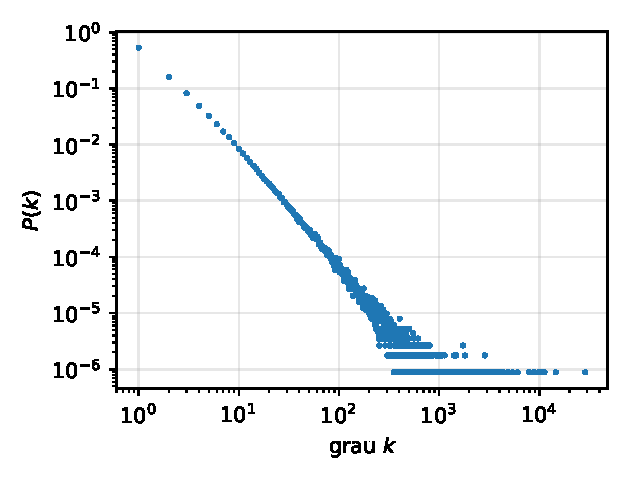
\includegraphics[width=\linewidth]{../parte1/resultados/fig/graus.pdf}}{\TODO{figura graus.pdf}}
  \caption{Distribuição de graus $P(k)$ em escala log-log.}
  \Description{Gráfico log-log da fração de vértices em função do grau.}
  \label{fig:graus}
\end{figure}

\begin{figure}[h]
  \centering
  \IfFileExists{../parte1/resultados/fig/visualizacao.pdf}{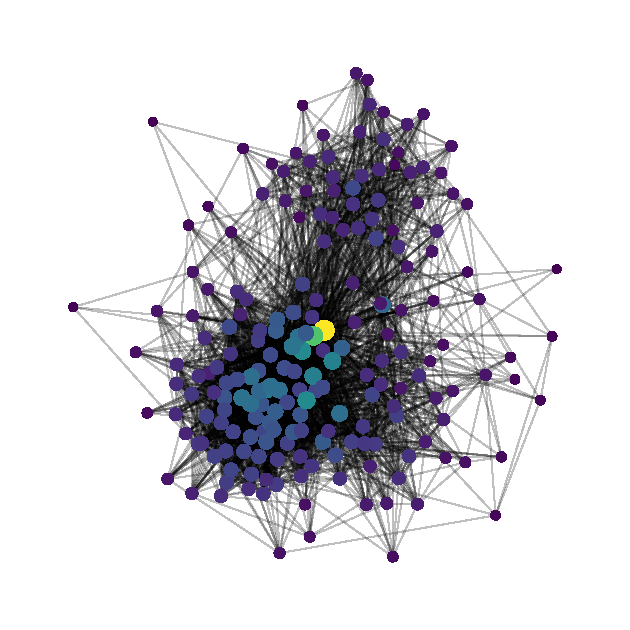
\includegraphics[width=0.8\linewidth]{../parte1/resultados/fig/visualizacao.pdf}}{\TODO{figura visualizacao.pdf}}
  \caption{Subgrafo reduzido ao redor do vértice de maior grau; tamanho e cor dos nós indicam o grau.}
  \Description{Visualização de um subgrafo com poucos hubs conectados a muitos vértices de grau baixo.}
  \label{fig:vis}
\end{figure}

%% =====================================================================
\section{Parte II - Algoritmos da Disciplina}
\label{sec:parte2}
As Tabelas~\ref{tab:complexidade} e~\ref{tab:tempos} e a Figura~\ref{fig:tempos} reúnem os resultados nos subgrafos. Os expoentes ajustados ficaram entre 1,04 e 1,14 para os algoritmos de custo $O(V+E)$ (BFS, DFS, eulerianidade, Tarjan), entre 0,96 e 1,11 para Dijkstra, Kruskal e Prim, e em 0,59 (Bellman-Ford) e 0,92 (Floyd-Warshall), todos com $R^2\ge0{,}989$.

\begin{table}
  \caption{Complexidade teórica e expoente observado $b$ do ajuste $t\propto f(V,E)^b$ (quanto mais próximo de 1, maior a aderência).}
  \label{tab:complexidade}
  \small
  \tabela{../parte2/resultados/tab_complexidade.tex}{python -m parte2}
\end{table}

\begin{table*}
  \caption{Tempos de execução observados (média, desvio padrão e IC95\%).}
  \label{tab:tempos}
  \small
  \tabela{../parte2/resultados/tab_tempos.tex}{python -m parte2}
\end{table*}

\begin{figure}[h]
  \centering
  \IfFileExists{../parte2/resultados/fig/tempos.pdf}{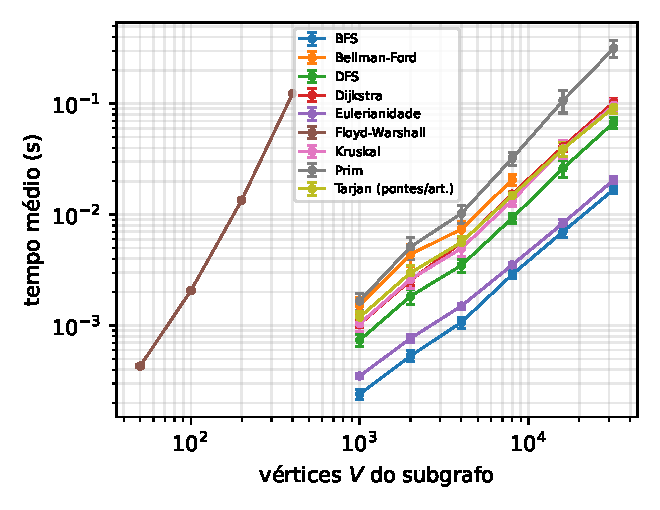
\includegraphics[width=\linewidth]{../parte2/resultados/fig/tempos.pdf}}{\TODO{figura tempos.pdf}}
  \caption{Tempo médio com IC95\% em função do tamanho do subgrafo (log-log).}
  \Description{Curvas de tempo por algoritmo em escala log-log, crescentes com o número de vértices.}
  \label{fig:tempos}
\end{figure}

\paragraph{Execução no grafo completo.} Pela distribuição de graus da Parte~I, 806\,868 vértices (71,1\%) têm grau ímpar; como um grafo euleriano (ciclo ou caminho) admite no máximo dois, o grafo \textbf{não} é euleriano. No grafo completo ($R=5$, $t$ de Student), BFS levou $0{,}387\pm0{,}009$~s, DFS $1{,}012\pm0{,}008$~s, a verificação de eulerianidade $0{,}509\pm0{,}034$~s, Tarjan $1{,}727\pm0{,}109$~s e Kruskal $0{,}719\pm0{,}022$~s (IC95\%). O grafo tem 667\,090 pontes (22,3\% das arestas) e 223\,409 pontos de articulação (19,7\% dos vértices), e a árvore geradora tem 1\,134\,889 arestas ($n-1$, como esperado em grafo conexo com pesos unitários).

%% =====================================================================
\section{Parte III - Análise Estrutural Avançada}
\label{sec:parte3}

\subsection{Propriedade \emph{small-world}}
A Tabela~\ref{tab:sw} compara o grafo real com o aleatório. O grafo aleatório simulado tem, na sua maior componente, 1\,128\,880 vértices e 2\,987\,531 arestas. O caminho médio é $5{,}34\pm0{,}09$ no grafo real e $8{,}55\pm0{,}03$ no aleatório (teórico 8,39); a clusterização é $0{,}0796\pm0{,}0031$ no real (estimativa amostral; valor exato 0,0808 da Parte~I) e $3{,}6\times10^{-6}$ no aleatório. Resultam $L/L_{rand}=0{,}62$, $C/C_{rand}\approx22\,300$ e $\sigma\approx3{,}6\times10^{4}$.

\begin{table}
  \caption{Teste de \emph{small-world} na maior componente.}
  \label{tab:sw}
  \small
  \tabela{../parte3/resultados/tab_smallworld.tex}{python -m parte3.smallworld}
\end{table}

\subsection{Lei de potência na distribuição de graus}
O MLE dá $\gamma=2{,}14\pm0{,}003$ com $k_{min}=8$; a cauda ($k\ge8$) contém 119\,156 vértices, cerca de 10,5\% do total, e a distância de KS é 0,009. A regressão log-log da CCDF ($k\ge5$) dá $\gamma=2{,}43$ com $R^2=0{,}991$ (Tabela~\ref{tab:pl} e Figura~\ref{fig:pl}).

\begin{table}
  \caption{Ajuste de lei de potência.}
  \label{tab:pl}
  \small
  \tabela{../parte3/resultados/tab_potencia.tex}{python -m parte3.potencia}
\end{table}

\begin{figure}[h]
  \centering
  \IfFileExists{../parte3/resultados/fig/potencia.pdf}{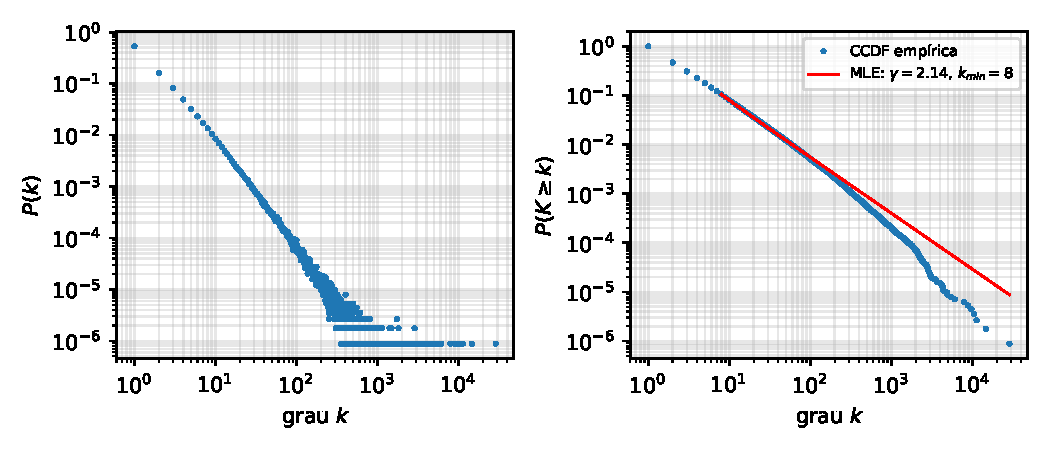
\includegraphics[width=\linewidth]{../parte3/resultados/fig/potencia.pdf}}{\TODO{figura potencia.pdf}}
  \caption{$P(k)$ e CCDF em escala log-log, com o ajuste por máxima verossimilhança.}
  \Description{Dois gráficos log-log: distribuição de graus e CCDF com reta de ajuste.}
  \label{fig:pl}
\end{figure}

\subsection{Robustez}
A Tabela~\ref{tab:rob} e a Figura~\ref{fig:rob} resumem os cenários. Foram removidos $r=56\,745$ vértices. Na remoção aleatória a maior componente retém $S=0{,}915\pm0{,}002$ do grafo, surgem cerca de 32\,800 componentes e 2,7\% de vértices isolados, e as distâncias quase não mudam (caminho médio 5,24 contra 5,19). Nos ataques direcionados, $S$ cai para 0,295 (grau) e 0,253 (PageRank), o número de componentes passa de 540\,000 e o caminho médio sobe para $\approx22$, com 43--47\% de isolados.

\begin{table*}
  \caption{Robustez à remoção de 5\% dos vértices.}
  \label{tab:rob}
  \small
  \tabela{../parte3/resultados/tab_robustez.tex}{python -m parte3.robustez}
\end{table*}

\begin{figure*}[h]
  \centering
  \IfFileExists{../parte3/resultados/fig/robustez.pdf}{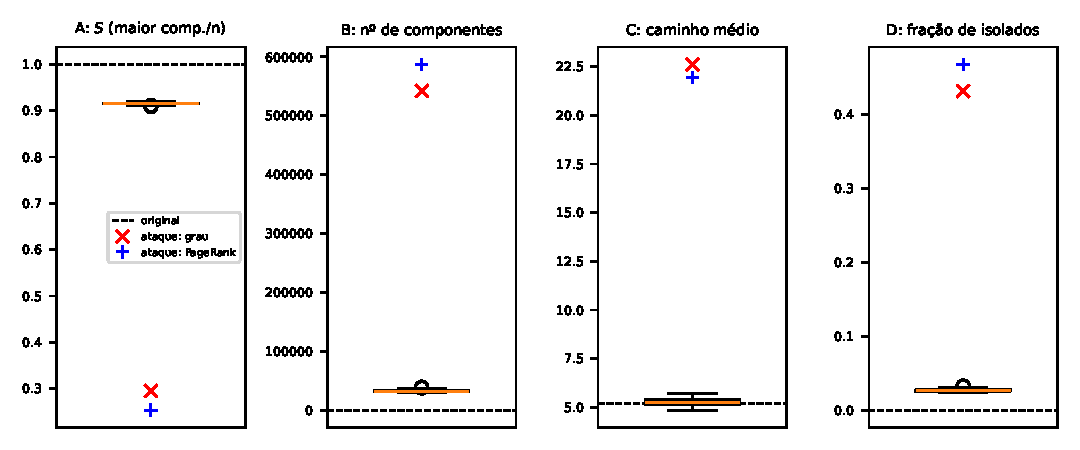
\includegraphics[width=0.85\textwidth]{../parte3/resultados/fig/robustez.pdf}}{\TODO{figura robustez.pdf}}
  \caption{Métricas após a remoção aleatória (boxplots, $T$ repetições) e após ataques por grau e PageRank (marcadores); linha tracejada = grafo original.}
  \Description{Quatro painéis com boxplots das métricas A a D e marcadores dos ataques direcionados.}
  \label{fig:rob}
\end{figure*}

\subsection{Descoberta mais interessante}
O mais interessante é que uma mesma propriedade explica a força e a fragilidade da rede. Os \emph{hubs} (cauda com $\gamma\approx2{,}1$) mantêm o caminho médio em 5,3 saltos, menor que o de um grafo aleatório equivalente (8,6), e o diâmetro em 24 mesmo com 1,1 milhão de vértices. Mas é por eles que tudo passa: remover só 5\% dos vértices por grau deixa apenas 29\% do grafo conectado, enquanto 5\% aleatórios deixam 91\%.

Há ainda um efeito de composição: mais da metade dos usuários tem um único amigo e pendura-se em algum \emph{hub}. Por isso a remoção aleatória isola quase exatamente a fração prevista (2,7\%), enquanto o ataque aos poucos vértices centrais isola 43\% de uma vez.

\subsection{Aproximação a modelos clássicos}
\emph{Erdős--Rényi}: com o mesmo grau médio, o grau seguiria uma Poisson de média 5,3, sem vértices de grau na casa de milhares, e $C\approx4{,}6\times10^{-6}$; o grafo real tem grau máximo 28\,754 e $C=0{,}081$, logo não se aproxima de ER. \emph{Watts--Strogatz}: reproduz $C$ alto e $L$ baixo, mas com graus homogêneos, o que contradiz a cauda pesada observada. \emph{Barabási--Albert} \cite{barabasi1999}: gera cauda de lei de potência e $L$ curto, mas com $\gamma=3$ e $C$ muito baixo; a rede real tem $\gamma\approx2{,}1$--$2{,}4$ e $C$ bem maior. O modelo mais próximo é, portanto, o de ligação preferencial, mas seria preciso um mecanismo adicional de fechamento de triângulos para explicar a clusterização.

%% =====================================================================
\section{Discussão Crítica}
\label{sec:discussao}
Esta seção separa o que os resultados indicam (Seção~\ref{sec:interpretacao}) do que limita a confiança nessas conclusões (Seção~\ref{sec:limitacoes}).

\subsection{Interpretação dos Resultados}
\label{sec:interpretacao}
\paragraph{Parte I.} A densidade é de apenas $4{,}6\times10^{-6}$: o grafo é extremamente esparso. O grau médio ($5{,}27$) esconde uma distribuição muito assimétrica: a mediana é 1 (53,1\% dos vértices têm um único amigo), enquanto o grau máximo é 28\,754, cerca de 5\,400 vezes a média, e 5\,821 vértices têm grau $\geq100$. Esses \emph{hubs} organizam a conectividade. O diâmetro (24) e o raio (12) são pequenos para mais de um milhão de vértices e o caminho médio é ainda menor ($5{,}36\pm0{,}12$): pares típicos ficam a cerca de cinco saltos, e os 24 saltos são casos extremos. Como $\mathrm{diam}\le 2\,\mathrm{raio}$ e o raio é no máximo 12, o diâmetro encontrado (24) é de fato exato e, como $\mathrm{raio}\ge\mathrm{diam}/2$, o raio também é exatamente 12. A clusterização média é 0,081, e há 3\,056\,386 triângulos: apesar da esparsidade, os amigos de um usuário têm probabilidade alta, em comparação com um grafo aleatório, de serem amigos entre si.

\paragraph{Parte II.} Os algoritmos de custo $O(V+E)$ (BFS, DFS, eulerianidade, Tarjan) apresentam expoente entre 1,04 e 1,14, e Dijkstra ($O((V+E)\log V)$), Kruskal e Prim ficam entre 0,96 e 1,11, todos com $R^2\ge0{,}997$: o tempo observado cresce de forma compatível com a teoria (o fator $\log V$ varia pouco nessa faixa e é absorvido pelo ajuste). Diferenças de constante entre eles, por exemplo Prim ser cerca de três vezes mais lento que Kruskal em $V=32\,000$, vêm da implementação em Python, não da ordem assintótica. Dois casos divergem: Bellman-Ford tem expoente 0,59, bem abaixo do $O(VE)$ teórico, porque a implementação encerra quando uma passada não relaxa nenhuma aresta; em grafos de diâmetro pequeno isso ocorre após poucas passadas, e o custo real se aproxima de $O(D\cdot E)$, onde $D$ é o número de passadas. Em Floyd-Warshall (0,92), a sobrecarga fixa ainda pesa frente ao termo cúbico nos tamanhos medidos.

\paragraph{Small-world.} Há forte indício de \emph{small-world}. A clusterização do grafo real (0,0796) é cerca de $2\times10^{4}$ vezes a do grafo aleatório simulado ($C/C_{rand}\approx 22\,300$) e, com o valor teórico $C_{rand}\approx 4{,}6\times10^{-6}$, ainda ficaria em $\approx1{,}7\times10^{4}$. O caminho médio ($5{,}34$) não é apenas da mesma ordem que o aleatório ($8{,}55$; teórico $8{,}39$): é \emph{menor} ($L/L_{rand}=0{,}62$). Isso é esperado em redes com \emph{hubs}, que funcionam como atalhos. Na prática, informação e influência alcançam qualquer usuário em cerca de cinco saltos, com agrupamento local forte, típico de comunidades de amigos.

\paragraph{Lei de potência.} O valor da regressão ($\gamma=2{,}43$) é maior que o do MLE ($2{,}14$): a regressão sobre a CCDF é sabidamente enviesada em caudas ruidosas, e por isso se prefere o MLE. Em ambos os casos $2<\gamma<3$, faixa típica de redes livres de escala, em que a média é finita mas a variância teórica diverge; é o que permite \emph{hubs} como o de grau 28\,754.

\paragraph{Robustez.} Os 2,7\% de vértices isolados na remoção aleatória são coerentes com a estrutura: 53,1\% dos vértices têm grau 1 e, com 5\% de remoção, cerca de $0{,}531\times0{,}05\approx2{,}7\%$ perdem seu único vizinho. Como $S_{rand}\gg S_{cent}$ e $c_{cent}\gg c_{rand}$, a rede é \textbf{robusta a falhas aleatórias e vulnerável a ataques direcionados}, padrão típico de redes com \emph{hubs}. O PageRank causa dano um pouco maior que o grau.

\subsection{Limitações}
\label{sec:limitacoes}
\paragraph{Dados e Parte I.} (i) O SNAP distribui apenas a maior componente conexa; a componente única e a ausência de vértices isolados são consequência desse recorte, e não uma propriedade da rede completa do YouTube. Todas as conclusões de conectividade e de robustez valem para essa componente. (ii) A única medida de caminhos estimada é o caminho médio ($\pm0{,}12$); as demais medidas numéricas da Tabela~\ref{tab:estrutural} são exatas. (iii) A visualização mostra apenas 200 vértices em torno do maior \emph{hub} e serve para ilustrar a estrutura de \emph{hubs}, não para inferir propriedades do grafo inteiro.

\paragraph{Parte II.} (i) Os subgrafos são bolas BFS em torno de vértices aleatórios, e não amostras uniformes; a razão $E/V$ cresce de 2,3 ($V=1\,000$) a 5,6 ($V=32\,000$), contra 2,6 no grafo completo, e por isso o ajuste usa $f(V,E)$ e não apenas $V$. (ii) Os pesos são sintéticos, de modo que os resultados de Dijkstra, Bellman-Ford, Kruskal e Prim não refletem pesos reais. (iii) Os tempos vêm de implementações em Python, em uma única máquina, e expoentes acima de 1 (como 1,10 e 1,14 para BFS e DFS) podem refletir efeitos de \emph{cache} e de alocação de memória, que não foram investigados. (iv) Floyd-Warshall foi medido só até $V=400$, o que torna o seu expoente pouco informativo. (v) No grafo completo foram medidos apenas cinco algoritmos, com $R=5$, o que alarga os IC95\% (daí o uso da $t$ de Student).

\paragraph{Small-world.} (i) A clusterização do grafo real foi estimada em uma amostra de 20\,000 vértices ($0{,}0796\pm0{,}0031$, contra o valor exato 0,0808), e o caminho médio por BFS amostradas. (ii) O $C_{rand}$ simulado vem de uma amostra com poucos triângulos e seu IC95\% ($\pm4{,}9\times10^{-6}$) é maior que o próprio valor; por isso o valor teórico é a referência mais estável e $\sigma$ ($\approx3{,}6\times10^{4}$; $\approx2{,}7\times10^{4}$ com o $C_{rand}$ teórico) deve ser lido como ordem de grandeza, não como valor preciso.

\paragraph{Lei de potência.} O erro-padrão do MLE (0,003) mede apenas a incerteza estatística condicionada ao modelo e ao $k_{min}$ escolhido, não a adequação da lei de potência. Como não foram feitos o teste de bondade de ajuste por \emph{bootstrap} nem a comparação com outras distribuições de cauda pesada, o resultado é um indício compatível com lei de potência, não uma prova. Os 90\% de vértices abaixo de $k_{min}$ (inclusive os 53\% de grau 1) não seguem necessariamente a lei.

\paragraph{Robustez.} (i) As métricas de distância usam apenas 20 BFS; o caminho médio (5,19) e o diâmetro ($\ge17$) do grafo original são, portanto, estimativas mais ruidosas que as da Parte~I (5,36 e 24) e do teste de \emph{small-world} (5,34), e podem ser refinadas com mais BFS. (ii) O ataque usa ranking \emph{fixo}, calculado uma vez; um ataque adaptativo, que recalcula a centralidade a cada remoção, tende a ser mais danoso, e a betweenness não foi usada por ser inviável neste porte. (iii) O caminho médio de $\approx22$ após os ataques refere-se à maior componente remanescente, que tem apenas 25--30\% do grafo original.

%% =====================================================================
\section{Conclusão}
\label{sec:conclusao}
A rede \texttt{com-Youtube} é esparsa, de mundo pequeno (caminho médio 5,4, diâmetro 24, alta clusterização) e com distribuição de graus de cauda pesada. Essa combinação a torna robusta a falhas aleatórias, mas vulnerável à perda dos \emph{hubs}. Os algoritmos implementados tiveram tempo observado compatível com a complexidade teórica, com Bellman-Ford e Floyd-Warshall como exceções explicadas pelo encerramento antecipado e pela faixa pequena de tamanhos.

As principais limitações são: diâmetro, raio e caminho médio estimados por BFS amostradas; clusterização do teste de \emph{small-world} estimada em amostra; lei de potência sem teste de bondade de ajuste nem comparação com outras distribuições; e ataques com ranking fixo, sem recalcular a centralidade a cada remoção, nem betweenness. Como trabalhos futuros, propõe-se o teste por \emph{bootstrap}, o ataque adaptativo e a comparação com modelos geradores que incluam fechamento de triângulos.

\begin{acks}
Agradeço ao professor Bruno pela ótima proposta de Trabalho Prático e a chance que proporcionou para os seus alunos se desenvolverem durante a matéria. Foi uma ótima experiência para todos assistir às suas aulas e  desenvolver habilidades pertinentes à pesquisa científica durante os seminários.
\end{acks}

\bibliographystyle{ACM-Reference-Format}
\bibliography{refs}

\end{document}
\endinput
